\documentclass{beamer}
\usepackage{tikz}
\usepackage{CJKutf8}
\usepackage{ragged2e}
\justifying\let\raggedright\justifying
\usepackage{graphicx}
\setbeamertemplate{theorems}[numbered]
\begin{document}
\begin{CJK}{UTF8}{gbsn}
\newtheorem*{Exercise}{习题}
\newtheorem{Thm}{定理}[section]
\newtheorem*{Thm1}{定理1.1}
\newtheorem*{Thm2}{定理4.1}
\newtheorem*{Thm3}{定理4.5}
\newtheorem*{Thm4.5}{定理4.5}
\newtheorem{Cor}{推论}
\theoremstyle{definition}
\newtheorem{Def}{定义}[section]
\newtheorem*{Def1}{定义}
\newtheorem*{Thm4}{定理}
\theoremstyle{example}
\newtheorem*{Ex}{例:}
\date{}
\author{陈建文}

\title{第九章 平面图和图的着色}
\begin{frame}
  \titlepage
  
\end{frame}
\begin{frame}
  \frametitle{第九章 平面图和图的着色}
\end{frame}

\begin{frame}
  \frametitle{第九章 平面图和图的着色}
  \begin{enumerate}
  \item 平面图\\
\pause
在印刷电路的布线中,人们感兴趣的是要知道一个特定的电网络是否可以嵌入平面上。
\pause
\item 图的着色\\
% \pause
% \includegraphics[width=5cm,height=3cm]{Worldmap}
  \end{enumerate}
\end{frame}

% \begin{frame}
%   \frametitle{9.1 平面图及其欧拉公式}
%   \begin{definition9.1.1}
%     图$G$称为被嵌入平(曲)面$S$内,如果$G$的图解已画在$S$上,而且任何两条边均不相交(除可能在端点相交外)。
% 已嵌入平面内的图称平面图。如果一个图可以嵌入平面,则称此图是可平面的。
%   \end{definition9.1.1}
% \includegraphics[width=4cm,height=3cm]{k4}
% \end{frame}
\section{平面图及其欧拉公式}
\begin{frame}
    \centering
  \begin{minipage}{0.24\linewidth}
    \centering
    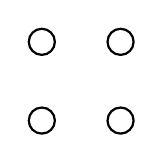
\begin{tikzpicture}[auto,
    specification/.style ={circle, draw, thick}]
   \node[specification] (A) at (0,0)  {};
   \node[specification] (B)  at (0,1)  {};
   \node[specification] (C)  at (1,1)  {};
   \node[specification] (D) at (1,0)  {};
 \end{tikzpicture}\\
 A
\end{minipage}\hfill 
  \begin{minipage}{0.24\linewidth}
    \centering
    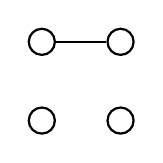
\begin{tikzpicture}[auto,
    specification/.style ={circle, draw, thick}]
   \node[specification] (A) at (0,0)  {};
   \node[specification] (B) at (0,1)  {};
   \node[specification] (C) at (1,1)  {};
   \node[specification] (D) at (1,0)  {};
   \draw[thick] (B) to  (C);
 \end{tikzpicture}\\
 B
\end{minipage}\hfill 
  \begin{minipage}{0.24\linewidth}
    \centering
    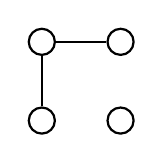
\begin{tikzpicture}[auto,
    specification/.style ={circle, draw, thick}]
   \node[specification] (A) at (0,0)  {};
   \node[specification] (B) at (0,1)  {};
   \node[specification] (C) at (1,1)  {};
   \node[specification] (D) at (1,0)  {};
   \draw[thick] (A) to  (B);
   \draw[thick] (B) to  (C);
 \end{tikzpicture}\\
 C
\end{minipage}\hfill 
  \begin{minipage}{0.24\linewidth}
    \centering
    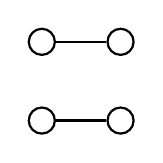
\begin{tikzpicture}[auto,
    specification/.style ={circle, draw, thick}]
   \node[specification] (A)  at (0,0)  {};
   \node[specification] (B)  at (0,1)  {};
   \node[specification] (C)  at (1,1)  {};
   \node[specification] (D) at (1,0)  {};
   \draw[thick] (B) to  (C);
   \draw[thick] (D) to  (A);
 \end{tikzpicture}\\
 D
\end{minipage}\hfill

\vspace*{0.5cm}
  \begin{minipage}{0.24\linewidth}
    \centering
    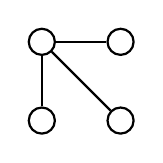
\begin{tikzpicture}[auto,
    specification/.style ={circle, draw, thick}]
   \node[specification] (A) at (0,0)  {};
   \node[specification] (B)  at (0,1)  {};
   \node[specification] (C)  at (1,1)  {};
   \node[specification] (D) at (1,0)  {};
   \draw[thick] (A) to (B);
   \draw[thick] (B) to (C);
      \draw[thick] (B) to (D);
 \end{tikzpicture}\\
 E
\end{minipage}\hfill
  \begin{minipage}{0.24\linewidth}
    \centering
    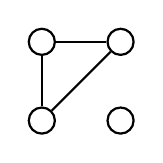
\begin{tikzpicture}[auto,
    specification/.style ={circle, draw, thick}]
   \node[specification] (A) at (0,0)  {};
   \node[specification] (B) at (0,1)  {};
   \node[specification] (C) at (1,1)  {};
   \node[specification] (D) at (1,0)  {};
   \draw[thick] (A) to  (B);
   \draw[thick] (B) to (C);
   \draw[thick] (C) to (A);
 \end{tikzpicture}\\
 F
\end{minipage}\hfill
  \begin{minipage}{0.24\linewidth}
    \centering
    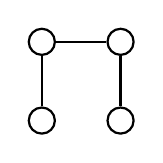
\begin{tikzpicture}[auto,
    specification/.style ={circle, draw, thick}]
   \node[specification] (A) at (0,0)  {};
   \node[specification] (B) at (0,1)  {};
   \node[specification] (C) at (1,1)  {};
   \node[specification] (D) at (1,0)  {};
   \draw[thick] (A) to  (B);
   \draw[thick] (B) to  (C);
      \draw[thick] (C) to (D);
 \end{tikzpicture}\\
 G
\end{minipage}\hfill 
  \begin{minipage}{0.24\linewidth}
    \centering
    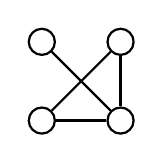
\begin{tikzpicture}[auto,
    specification/.style ={circle, draw, thick}]
   \node[specification] (A)  at (0,0)  {};
   \node[specification] (B)  at (0,1)  {};
   \node[specification] (C)  at (1,1)  {};
   \node[specification] (D) at (1,0)  {};
   \draw[thick] (A) to  (C);
   \draw[thick] (C) to  (D);
   \draw[thick] (D) to (A);
   \draw[thick] (B) to (D);
 \end{tikzpicture}\\
 H
\end{minipage}\hfill 

\vspace*{0.5cm}
\flushleft
  \begin{minipage}{0.24\linewidth}
    \centering
    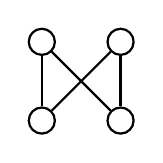
\begin{tikzpicture}[auto,
    specification/.style ={circle, draw, thick}]
   \node[specification] (A) at (0,0)  {};
   \node[specification] (B)  at (0,1)  {};
   \node[specification] (C)  at (1,1)  {};
   \node[specification] (D) at (1,0)  {};
   \draw[thick] (A) to (B);
   \draw[thick] (B) to (D);
   \draw[thick] (D) to (C);
      \draw[thick] (C) to (A);
 \end{tikzpicture}\\
 I
\end{minipage}
  \begin{minipage}{0.24\linewidth}
    \centering
    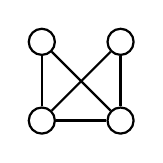
\begin{tikzpicture}[auto,
    specification/.style ={circle, draw, thick}]
   \node[specification] (A) at (0,0)  {};
   \node[specification] (B) at (0,1)  {};
   \node[specification] (C) at (1,1)  {};
   \node[specification] (D) at (1,0)  {};
   \draw[thick] (A) to  (B);
      \draw[thick] (C) to (D);
   \draw[thick] (D) to (A);
   \draw[thick] (A) to (C);
   \draw[thick] (B) to (D);
 \end{tikzpicture}\\
 J
\end{minipage} 
  \begin{minipage}{0.24\linewidth}
    \centering
    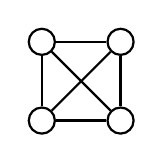
\begin{tikzpicture}[auto,
    specification/.style ={circle, draw, thick}]
   \node[specification] (A) at (0,0)  {};
   \node[specification] (B) at (0,1)  {};
   \node[specification] (C) at (1,1)  {};
   \node[specification] (D) at (1,0)  {};
   \draw[thick] (A) to  (B);
   \draw[thick] (B) to  (C);
      \draw[thick] (C) to (D);
   \draw[thick] (D) to (A);
   \draw[thick] (A) to (C);
   \draw[thick] (B) to (D);
 \end{tikzpicture}\\
 K
\end{minipage}  


\end{frame}
\begin{frame}
  \frametitle{9.1 平面图及其欧拉公式}
\pause
  \begin{Def}
    图$G$称为被嵌入平(曲)面$S$内,如果$G$的图解已画在$S$上,而且任意两条边均不相交(除可能在端点相交外)。
已嵌入平面内的图称为\alert{平面图}。如果一个图可以嵌入平面,则称此图为\alert{可平面}的。
\end{Def}
%   \begin{minipage}{0.45\linewidth}
% \includegraphics[width=4cm,height=3cm]{k4}    
%   \end{minipage}
%   \begin{minipage}{0.45\linewidth}
%     \includegraphics[width=4cm,height=3cm]{k4planar}
%   \end{minipage}
\end{frame}

\begin{frame}
  \frametitle{9.1 平面图及其欧拉公式}
%   \begin{definition9.1.1}
%     图$G$称为被嵌入平(曲)面$S$内,如果$G$的图解已画在$S$上,而且任何两条边均不相交(除可能在端点相交外)。
% 已嵌入平面内的图称平面图。如果一个图可以嵌入平面,则称此图是可平面的。
%   \end{definition9.1.1}
  \begin{minipage}{0.45\linewidth}
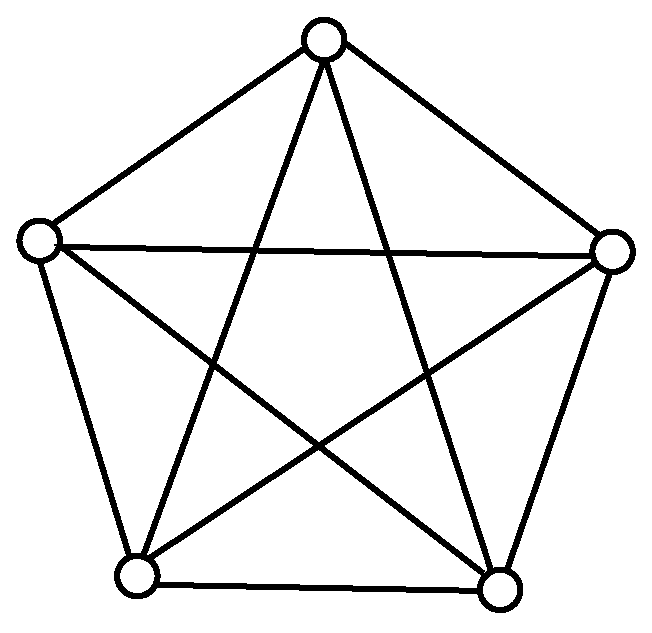
\includegraphics[width=4cm,height=3cm]{k5}    
  \end{minipage}
\pause
  \begin{minipage}{0.45\linewidth}
    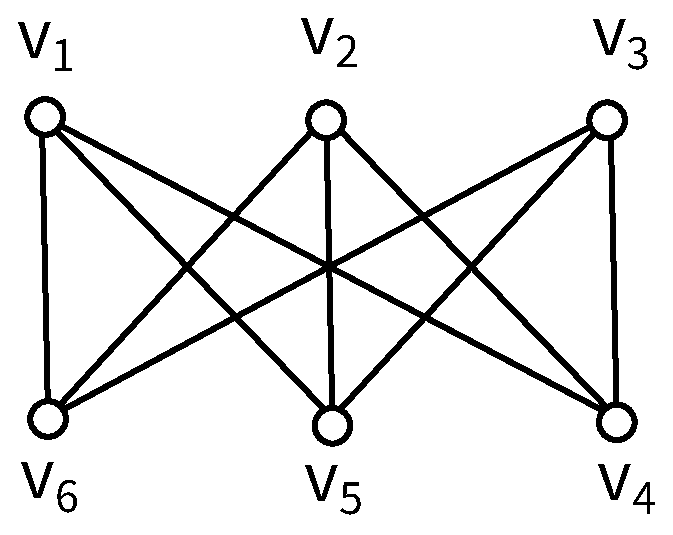
\includegraphics[width=4cm,height=3cm]{k33}
  \end{minipage}
\pause
  \begin{thebibliography}{99}
  \bibitem[Hopcroft, 1974]{Hopcropt1974}J. Hopcroft and R. Tarjan.
\newblock Efficient planarity testing.
\newblock Journal of the Association for Computing Machinery, 21(4):549-568, 1974.
  \end{thebibliography}
\pause
  \begin{thebibliography}{99}
  \bibitem[Boyer, 2004]{Boyer2004}J. Boyer and W. Myrvold.
\newblock On the Cutting Edge: Simplified O(n) Planarity by Edge Addition.
\newblock Journal of Grah algorithms and Applications, 8(3):241-273, 2004.
  \end{thebibliography}
\end{frame}
\begin{frame}
  \frametitle{9.1 平面图及其欧拉公式}
  \begin{Def}
    平面图$G$把平面分成了若干个区域,这些区域都是连通的,称之为$G$的\alert{面},其中无界的那个连通区域称为$G$的\alert{外部面},其余的连通区域称为$G$的\alert{内部面}。
  \end{Def}    
  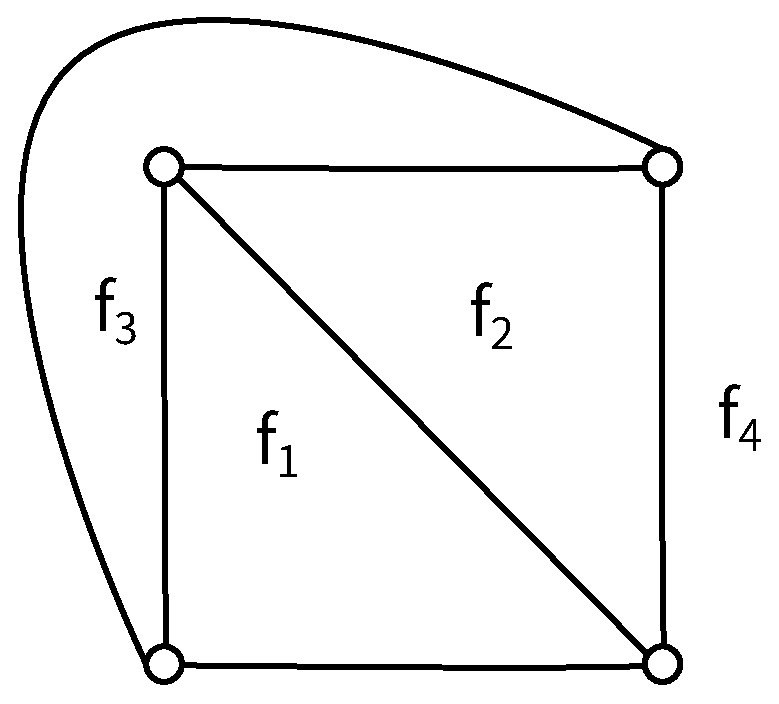
\includegraphics[width=4cm,height=3cm]{face}
\end{frame}
\begin{frame}
  \frametitle{9.1 平面图及其欧拉公式}
  \begin{Thm}
    如果有$p$个顶点$q$条边的平面连通图$G$有$f$个面,则
      $p - q + f = 2$
  \end{Thm}
\vspace{1cm}
\centering
    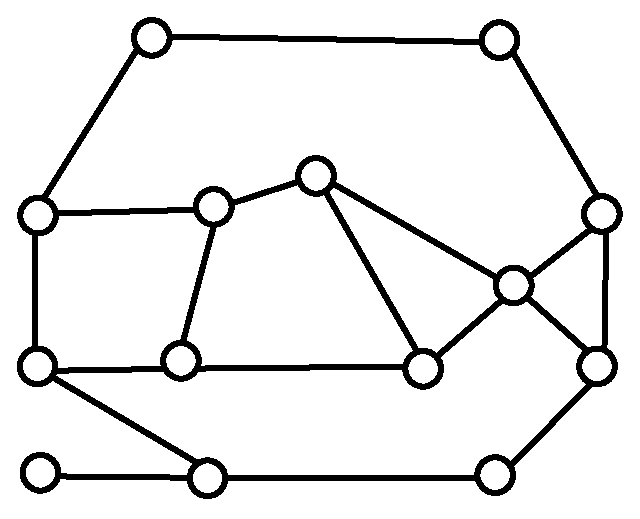
\includegraphics[width=4cm,height=3cm]{euler}
\end{frame}

\begin{frame}
  \frametitle{9.1 平面图及其欧拉公式}
  \begin{Thm1}
    如果有$p$个顶点$q$条边的平面连通图$G$有$f$个面,则
      $p - q + f = 2$
  \end{Thm1}
\vspace{1cm}
\centering
    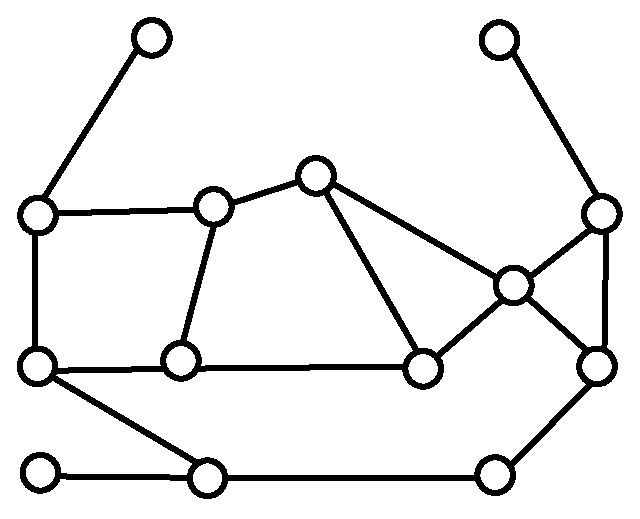
\includegraphics[width=4cm,height=3cm]{euler1}
\end{frame}
\begin{frame}
  \frametitle{9.1 平面图及其欧拉公式}
  \begin{Thm1}
    如果有$p$个顶点$q$条边的平面连通图$G$有$f$个面,则
      $p - q + f = 2$
  \end{Thm1}
\vspace{1cm}
\centering
    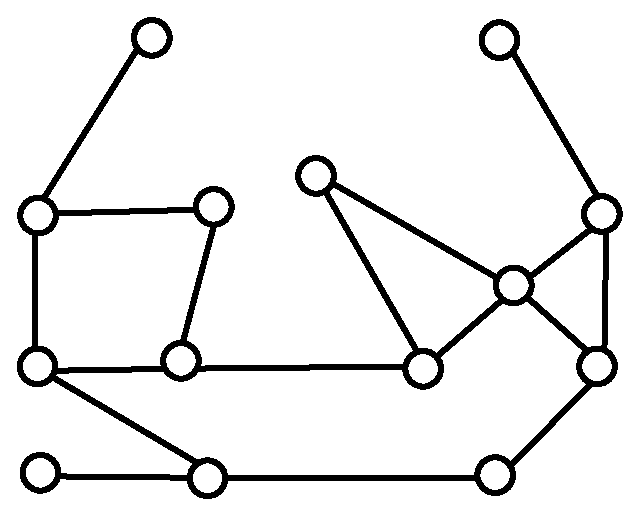
\includegraphics[width=4cm,height=3cm]{euler2}
\end{frame}
\begin{frame}
  \frametitle{9.1 平面图及其欧拉公式}
  \begin{Thm1}
    如果有$p$个顶点$q$条边的平面连通图$G$有$f$个面,则
      $p - q + f = 2$
  \end{Thm1}
\vspace{1cm}
\centering
    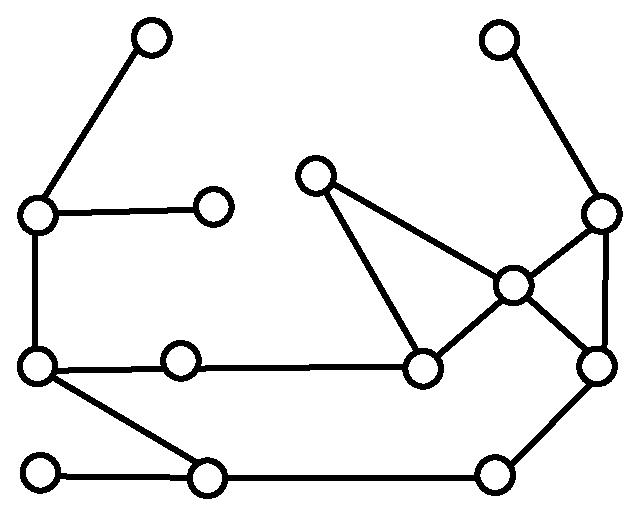
\includegraphics[width=4cm,height=3cm]{euler3}
\end{frame}
\begin{frame}
  \frametitle{9.1 平面图及其欧拉公式}
  \begin{Thm1}
    如果有$p$个顶点$q$条边的平面连通图$G$有$f$个面,则
      $p - q + f = 2$
  \end{Thm1}
\vspace{1cm}
\centering
    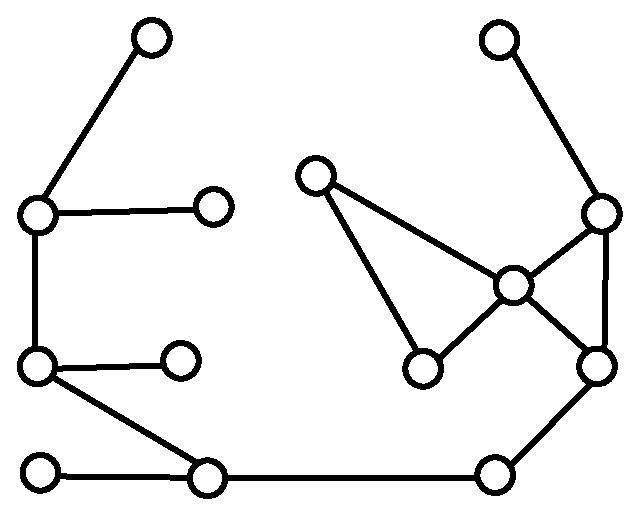
\includegraphics[width=4cm,height=3cm]{euler4}
\end{frame}
\begin{frame}
  \frametitle{9.1 平面图及其欧拉公式}
  \begin{Thm1}
    如果有$p$个顶点$q$条边的平面连通图$G$有$f$个面,则
      $p - q + f = 2$
  \end{Thm1}
\vspace{1cm}
\centering
    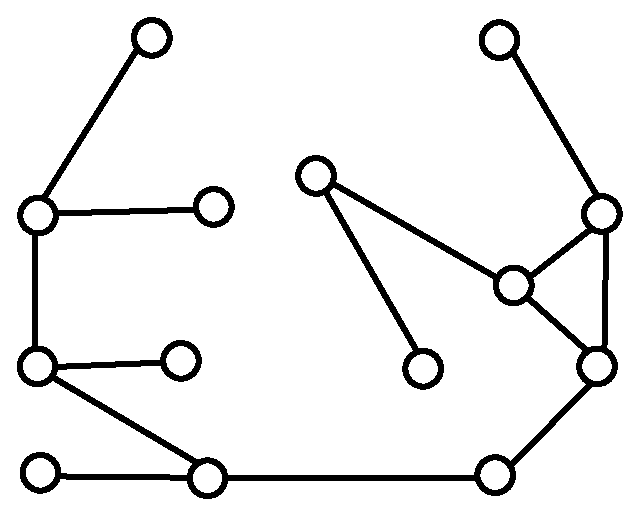
\includegraphics[width=4cm,height=3cm]{euler5}
\end{frame}

\begin{frame}
  \frametitle{9.1 平面图及其欧拉公式}
  \begin{Thm1}
    如果有$p$个顶点$q$条边的平面连通图$G$有$f$个面,则
      $p - q + f = 2$
  \end{Thm1}
\vspace{1cm}
\centering
    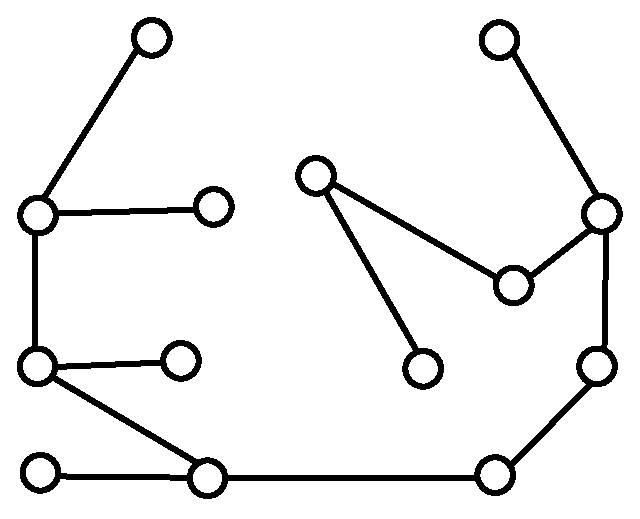
\includegraphics[width=4cm,height=3cm]{euler6}
\end{frame}

\begin{frame}
  \frametitle{9.1 平面图及其欧拉公式}
  \begin{Thm1}
    如果有$p$个顶点$q$条边的平面连通图$G$有$f$个面,则
      $p - q + f = 2$
  \end{Thm1}
\vspace{1cm}
\centering
    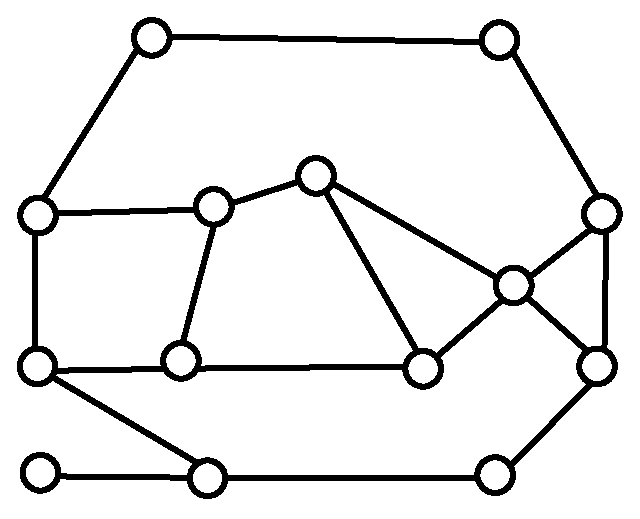
\includegraphics[width=4cm,height=3cm]{euler}
\end{frame}
\begin{frame}
  \frametitle{9.1 平面图及其欧拉公式}
  \begin{Thm1}
    如果有$p$个顶点$q$条边的平面连通图$G$有$f$个面,则
      $p - q + f = 2$
    \end{Thm1}
    \pause\begin{proof}[证明]
   \pause用数学归纳法证明,\pause施归纳于面数$f$。

  \pause(1)当$f=1$时,\pause $G$中无圈,\pause又因为$G$是连通的,\pause所以$G$是树。\pause从而
  $q=p-1$,\pause $p-q+f=2$成立。

  \pause(2)假设当$f=k(k\geq 1)$时结论成立,\pause往证当$f=k+1$时结论也成立。\pause假设$G$有$k+1$个面,\pause此时$G$至少有一个内部面,\pause从而有一个圈。\pause从这个圈上去掉一条边$x$,\pause则
  $G-x$就是一个有$p$个顶点,\pause$q-1$条边,\pause$k$个面的平面连通图。\pause由归纳假设,\pause对
  $G-x$结论成立,\pause即\[p-(q-1) + k =2\]
  \pause因此,\[p-q+ (k+1) =2\]
  \pause即当$f=k+1$时结论也成立。
\end{proof}

  
\end{frame}
\begin{frame}
  \frametitle{9.1 平面图及其欧拉公式}
  \begin{Cor}
    若平面图$G$有$p$个顶点$q$条边且每个面都是由长为$n$的圈围成的,则
    \begin{equation*}
      q = n(p-2)/(n-2)
    \end{equation*}
  \end{Cor}
\end{frame}
\begin{frame}
  \frametitle{9.1 平面图及其欧拉公式}
一个\alert{最大可平面图}是一个可平面图,对此可平面图中不能再加入边而不破坏其可平面性。
  \begin{Cor}
    设$G$为一个有$p$个顶点$q$条边的最大可平面图,$p \geq 3$,则$G$的每个面都为三角形,而且$q=3p-6$。
  \end{Cor}
\end{frame}
\begin{frame}
  \frametitle{9.1 平面图及其欧拉公式}
  \begin{Cor}
    设$G$为一个$(p,q)$可平面连通图,而且$G$的每个面都是由一个长为$4$的圈围成的,则$q=2p-4$。
  \end{Cor}
\end{frame}
\begin{frame}
  \frametitle{9.1 平面图及其欧拉公式}
  \begin{Cor}
    若$G$为一个有$p$个顶点$q$条边的可平面图,$p\geq 3$,则$q \leq 3p - 6$;进一步,若$G$中没有三角形,则$q \leq 2p -4$。
  \end{Cor}
  
      \pause
      \centering
    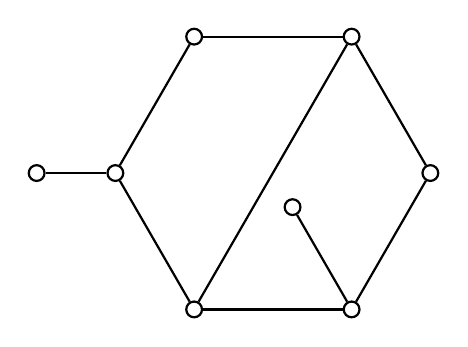
\begin{tikzpicture}[auto,
    specification/.style ={circle, draw, thick, inner sep = 0pt, minimum size=2mm}]
   \node[specification] (A)  at (0:2cm)  {};
   \node[specification] (B)  at (60:2cm)  {};
   \node[specification] (C)  at (120:2cm)  {};
   \node[specification] (D) at (180:2cm)  {};
   \node[specification] (E)  at (240:2cm)  {};   
   \node[specification] (F)  at (300:2cm)  {};   
   \node[specification] (G)  at (300:0.5cm)  {};
   \node[specification] (H)  at (180:3cm)  {};
   
   
   \draw[thick] (A) to  (B);
   \draw[thick] (B) to  (C);
   \draw[thick] (C) to  (D);
   \draw[thick] (D) to  (E);
   \draw[thick] (E) to  (F);
   \draw[thick] (F) to  (A);
   \draw[thick] (B) to  (E);
   \draw[thick] (F) to  (G);
   \draw[thick] (D) to  (H);   
 \end{tikzpicture}

\end{frame}
\begin{frame}
  \frametitle{9.1 平面图及其欧拉公式}
  \begin{Cor}
    $K_5$和$K_{3,3}$都不是可平面图。
  \end{Cor}
\vspace{1cm}
  \begin{minipage}{0.45\linewidth}
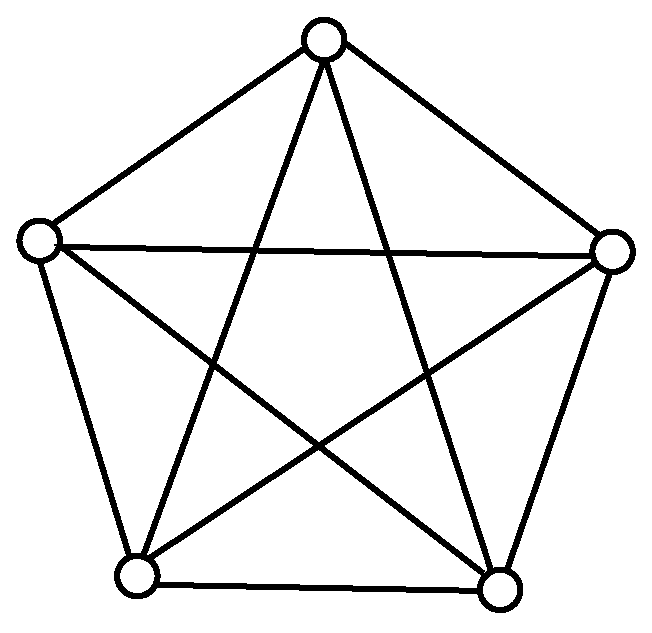
\includegraphics[width=4cm,height=3cm]{k5}    
  \end{minipage}
  \begin{minipage}{0.45\linewidth}
    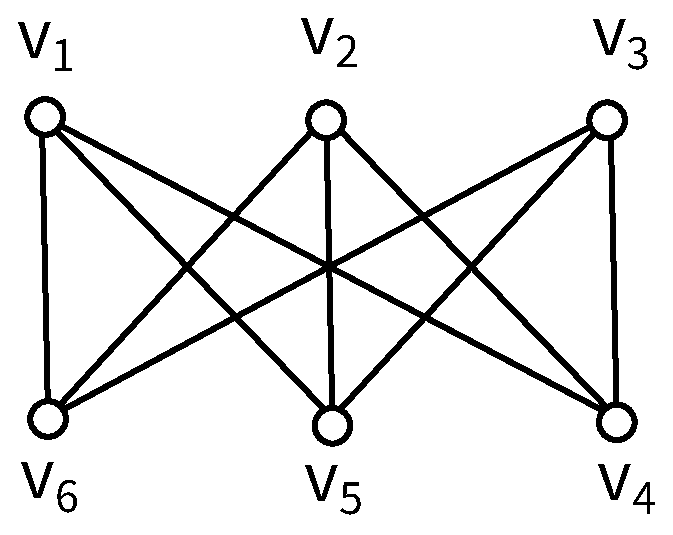
\includegraphics[width=4cm,height=3cm]{k33}
  \end{minipage}
\end{frame}
\begin{frame}
  \frametitle{9.1 平面图及其欧拉公式}
  \begin{Cor}
    每个可平面图$G$中顶点度的最小值不超过5,即$\delta (G) \leq 5$。
  \end{Cor}
\end{frame}
\begin{frame}
  \begin{Exercise}
    图$G$的最短圈的长度称为$G$的围长。如果$G$中无圈,则定义$G$的围长为无穷大。

    (1)证明:围长为$r$的平面连通图$G$中有
    \[q\leq r(p-2)/(r-2), r\geq 3\]

    (2)利用(1)证明Petersen图不是平面图。

    \centering
    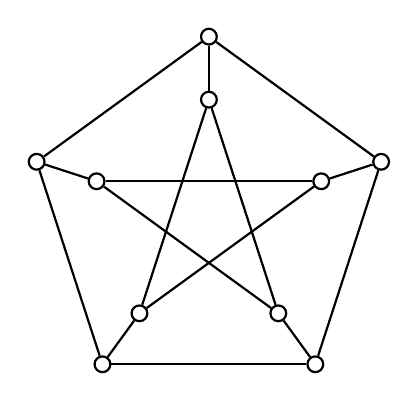
\begin{tikzpicture}[auto,
    specification/.style ={circle, draw, thick, inner sep = 0pt, minimum size=2mm}]
   \node[specification] (A)  at (18:2.3cm)  {};
   \node[specification] (B)  at (90:2.3cm)  {};
   \node[specification] (C)  at (162:2.3cm)  {};
   \node[specification] (D) at (234:2.3cm)  {};
   \node[specification] (E)  at (306:2.3cm)  {};
   \node[specification] (F)  at (18:1.5cm)  {};
   \node[specification] (G)  at (90:1.5cm)  {};
   \node[specification] (H)  at (162:1.5cm)  {};
   \node[specification] (I) at (234:1.5cm)  {};
   \node[specification] (J) at (306:1.5cm)  {};
   
   
   \draw[thick] (A) to  (B);
   \draw[thick] (B) to  (C);
   \draw[thick] (C) to  (D);
   \draw[thick] (D) to  (E);
   \draw[thick] (E) to  (A);
   \draw[thick] (A) to  (F);
   \draw[thick] (B) to  (G);
   \draw[thick] (C) to  (H);
   \draw[thick] (D) to  (I);
   \draw[thick] (E) to  (J);

   \draw[thick] (F) to  (H);
   \draw[thick] (H) to  (J);
   \draw[thick] (J) to  (G);
   \draw[thick] (G) to  (I);
   \draw[thick] (I) to  (F);
 \end{tikzpicture}

  \end{Exercise}
\end{frame}
% \begin{frame}
%   \frametitle{9.1 平面图及其欧拉公式}
%   \begin{Exercise}
%     设$G$为一个有$p$个顶点的平面图,$p \geq 4$。证明:$G$中有4个度不超过5的顶点。
%   \end{Exercise}
% \end{frame}
% \begin{frame}
%   \frametitle{9.1 平面图及其欧拉公式}
%   \begin{Exercise}
%     设$G$为一个有$k$个支的平面图。若$G$的顶点数、边数、面数分别为$p$,$q$和$f$,试证:
%     \begin{equation*}
%       p - q + f = k + 1
%     \end{equation*}
%   \end{Exercise}
% \end{frame}

% \begin{frame}
%   \frametitle{9.1 平面图及其欧拉公式}
%   \begin{Exercise}
%     若$G$为顶点数$p > 11$的可平面图,试证$G^c$不是可平面图。
%   \end{Exercise}
% \end{frame}
% \begin{frame}
%   \frametitle{9.1 平面图及其欧拉公式}
%   \begin{Exercise}
%     设$S = \{x_1, x_2, \ldots, x_n\}$ 为平面上$n$个顶点的集合,$n \geq 3$, 其中任意两个顶点的距离至少为1。证明:$S$中至多有$3n-6$对顶点,其距离为1。
%   \end{Exercise}
% \end{frame}
% \begin{frame}
%   \frametitle{9.1 平面图及其欧拉公式}
%   \begin{Exercise}
%     证明:不存在7条棱的凸多面体。
%   \end{Exercise}
% \end{frame}
\section{非哈密顿平面图}

\begin{frame}
  \frametitle{9.2 非哈密顿平面图}
  \begin{Thm}
    设$G=(V,E)$为一个$(p,q)$平面哈密顿图,$C$为$G$的哈密顿圈。
    令$f_i$为$C$的内部由$i$条边围成的面的个数,$g_i$为$C$的外部$i$条边围成的面的个数,则
    \begin{align}
      &1 \cdot f_3 + 2 \cdot f_4 + 3 \cdot f_5 + \cdots = \sum_{i=3}^p(i-2)f_i = p - 2;\\
      &1 \cdot g_3 + 2 \cdot g_4 + 3 \cdot g_5 + \cdots = \sum_{i=3}^p(i-2)g_i = p - 2;\\
      &1 \cdot (f_3 - g_3) + 2 \cdot (f_4 - g_4) + 3 \cdot (f_5 - g_5) + \cdots = \sum_{i=3}^p(i-2)(f_i - g_i) = 0
    \end{align}
  \end{Thm}
\end{frame}


\begin{frame}
    \centering
    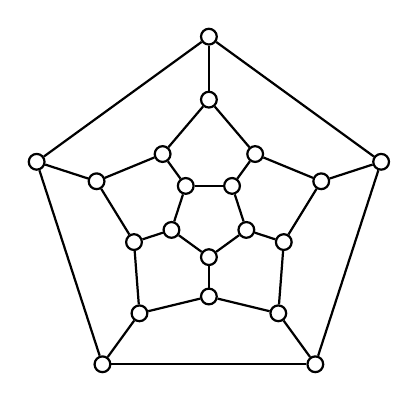
\begin{tikzpicture}[auto,
    specification/.style ={circle, draw, thick, inner sep = 0pt, minimum size=2mm}]
   \node[specification] (A)  at (18:2.3cm)  {};
   \node[specification] (B)  at (90:2.3cm)  {};
   \node[specification] (C)  at (162:2.3cm)  {};
   \node[specification] (D) at (234:2.3cm)  {};
   \node[specification] (E)  at (306:2.3cm)  {};
   \node[specification] (F)  at (18:1.5cm)  {};
   \node[specification] (G)  at (90:1.5cm)  {};
   \node[specification] (H)  at (162:1.5cm)  {};
   \node[specification] (I) at (234:1.5cm)  {};
   \node[specification] (J)  at (306:1.5cm)  {};
   \node[specification] (K)  at (-18:1.0cm)  {};
   \node[specification] (L)  at (-90:1.0cm)  {};
   \node[specification] (M)  at (-162:1.0cm)  {};
   \node[specification] (N) at (-234:1.0cm)  {};
   \node[specification] (O)  at (-306:1.0cm)  {};
   \node[specification] (P)  at (-18:0.5cm)  {};
   \node[specification] (Q)  at (-90:0.5cm)  {};
   \node[specification] (R)  at (-162:0.5cm)  {};
   \node[specification] (S) at (-234:0.5cm)  {};
   \node[specification] (T)  at (-306:0.5cm)  {};
   
   
   \draw[thick] (A) to  (B);
   \draw[thick] (B) to  (C);
   \draw[thick] (C) to  (D);
   \draw[thick] (D) to  (E);
   \draw[thick] (E) to  (A);
   \draw[thick] (A) to  (F);
   \draw[thick] (B) to  (G);
   \draw[thick] (C) to  (H);
   \draw[thick] (D) to  (I);
   \draw[thick] (E) to  (J);

   \draw[thick] (F) to  (O);
   \draw[thick] (O) to  (G);
   \draw[thick] (G) to  (N);
   \draw[thick] (N) to  (H);
   \draw[thick] (H) to  (M);
   \draw[thick] (M) to  (I);
   \draw[thick] (I) to  (L);
   \draw[thick] (L) to  (J);
   \draw[thick] (J) to  (K);
   \draw[thick] (K) to  (F);

   \draw[thick] (P) to  (K);
   \draw[thick] (Q) to  (L);
   \draw[thick] (R) to  (M);
   \draw[thick] (S) to  (N);
   \draw[thick] (T) to  (O);

   \draw[thick] (P) to  (Q);
   \draw[thick] (Q) to  (R);
   \draw[thick] (R) to  (S);
   \draw[thick] (S) to  (T);
   \draw[thick] (T) to  (P);
 \end{tikzpicture}

\end{frame}
\begin{frame}
  \frametitle{9.2 非哈密顿平面图}
  \centering
  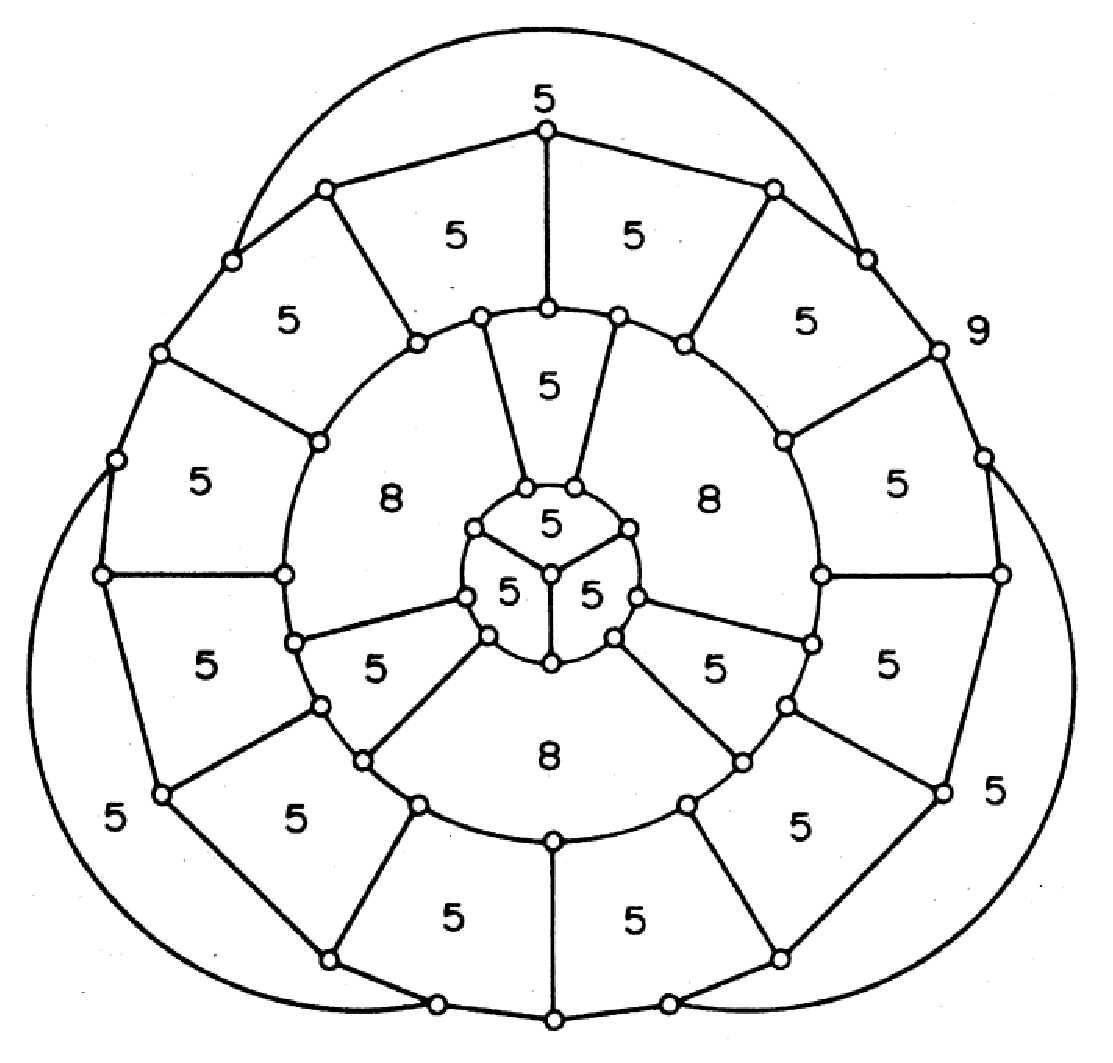
\includegraphics[width=7cm, height=6cm]{grinberg}
\end{frame}
\begin{frame}
  \frametitle{9.2 非哈密顿平面图}
  \centering
  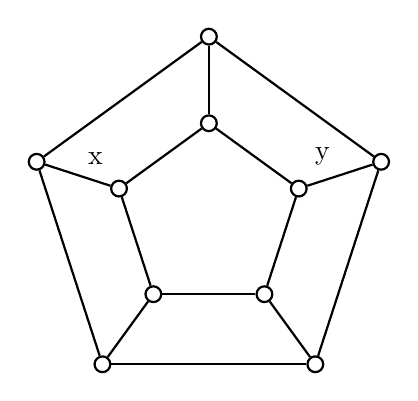
\begin{tikzpicture}[auto,
    specification/.style ={circle, draw, thick, inner sep = 0pt, minimum size=2mm}]
   \node[specification] (A)  at (18:2.3cm)  {};
   \node[specification] (B)  at (90:2.3cm)  {};
   \node[specification] (C)  at (162:2.3cm)  {};
   \node[specification] (D) at (234:2.3cm)  {};
   \node[specification] (E)  at (306:2.3cm)  {};
   \node[specification] (F)  at (18:1.2cm)  {};
   \node[specification] (G)  at (90:1.2cm)  {};
   \node[specification] (H)  at (162:1.2cm)  {};
   \node[specification] (I) at (234:1.2cm)  {};
   \node[specification] (J) at (306:1.2cm)  {};
   
   
   \draw[thick] (A) to  (B);
   \draw[thick] (B) to  (C);
   \draw[thick] (C) to  (D);
   \draw[thick] (D) to  (E);
   \draw[thick] (E) to  (A);
   \draw[thick] (F) to  (G);
   \draw[thick] (G) to  (H);
   \draw[thick] (H) to  (I);
   \draw[thick] (I) to  (J);
   \draw[thick] (J) to  (F);

   \draw[thick] (A) to  node[swap] {y} (F);
   \draw[thick] (B) to  (G);
   \draw[thick] (C) to node {x}   (H);
   \draw[thick] (D) to  (I);
   \draw[thick] (E) to  (J);
 \end{tikzpicture}
\end{frame}

\begin{frame}
  \frametitle{9.2 非哈密顿平面图}
  \centering
    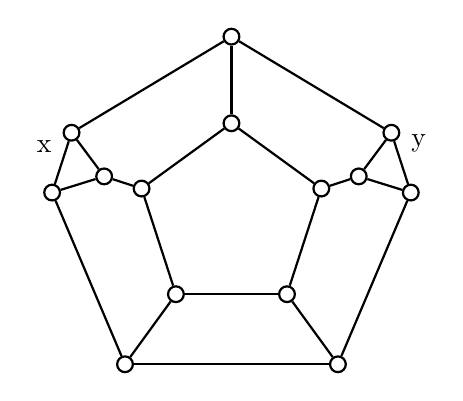
\begin{tikzpicture}[auto,
      specification/.style ={circle, draw, thick, inner sep = 0pt, minimum size=2mm}]
   \node[specification] (A1)  at (8:2.3cm)  {};
   
   \node[specification] (A)  at (18:1.7cm)  {};
   \node[specification] (A2)  at (28:2.3cm)  {};

   \node[specification] (B)  at (90:2.3cm)  {};
   \node[specification] (C1)  at (152:2.3cm)  {};   
   \node[specification] (C)  at (162:1.7cm)  {};
   \node[specification] (C2)  at (172:2.3cm)  {};

   \node[specification] (D) at (234:2.3cm)  {};
   \node[specification] (E)  at (306:2.3cm)  {};
   \node[specification] (F)  at (18:1.2cm)  {};
   \node[specification] (G)  at (90:1.2cm)  {};
   \node[specification] (H)  at (162:1.2cm)  {};
   \node[specification] (I) at (234:1.2cm)  {};
   \node[specification] (J) at (306:1.2cm)  {};


   \draw[thick] (A) to  (A1);
   \draw[thick] (A) to  (A2);
   \draw[thick] (A1) to node[swap] {y}  (A2);   
   \draw[thick] (A2) to  (B);
   \draw[thick] (B) to  (C1);

   \draw[thick] (C) to  (C1);
   \draw[thick] (C) to  (C2);
   \draw[thick] (C1) to node[swap] {x} (C2);
   \draw[thick] (C2) to  (D);
   \draw[thick] (D) to  (E);
   \draw[thick] (E) to  (A1);
   \draw[thick] (F) to  (G);
   \draw[thick] (G) to  (H);
   \draw[thick] (H) to  (I);
   \draw[thick] (I) to  (J);
   \draw[thick] (J) to  (F);

   \draw[thick] (A) to  (F);
   \draw[thick] (B) to  (G);
   \draw[thick] (C) to  (H);
   \draw[thick] (D) to  (I);
   \draw[thick] (E) to  (J);
 \end{tikzpicture}
\end{frame}

\begin{frame}
  \frametitle{9.2 非哈密顿平面图}
  \centering
      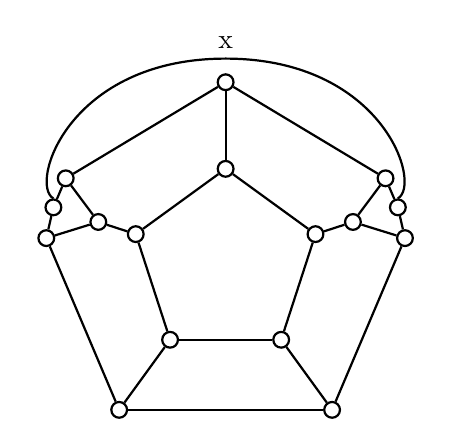
\begin{tikzpicture}[auto,
      specification/.style ={circle, draw, thick, inner sep = 0pt, minimum size=2mm}]
   \node[specification] (A1)  at (8:2.3cm)  {};
   \node[specification] (A3)  at (18:2.3cm)  {};   
   \node[specification] (A)  at (18:1.7cm)  {};
   \node[specification] (A2)  at (28:2.3cm)  {};

   \node[specification] (B)  at (90:2.3cm)  {};
   \node[specification] (C1)  at (152:2.3cm)  {};
   \node[specification] (C3)  at (162:2.3cm)  {};

   \node[specification] (C)  at (162:1.7cm)  {};
   \node[specification] (C2)  at (172:2.3cm)  {};

   \node[specification] (D) at (234:2.3cm)  {};
   \node[specification] (E)  at (306:2.3cm)  {};
   \node[specification] (F)  at (18:1.2cm)  {};
   \node[specification] (G)  at (90:1.2cm)  {};
   \node[specification] (H)  at (162:1.2cm)  {};
   \node[specification] (I) at (234:1.2cm)  {};
   \node[specification] (J) at (306:1.2cm)  {};


   \draw[thick] (A) to  (A1);
   \draw[thick] (A) to  (A2);
   \draw[thick] (A1) to   (A3);
   \draw[thick] (A3) to   (A2);

   \draw[thick] (A2) to  (B);
   \draw[thick] (B) to  (C1);

   \draw[thick] (C) to  (C1);
   \draw[thick] (C) to  (C2);
   \draw[thick] (C1) to  (C3);
   \draw[thick] (C3) to  (C2);
   \draw[thick] (C2) to  (D);
   \draw[thick] (D) to  (E);
   \draw[thick] (E) to  (A1);
   \draw[thick] (F) to  (G);
   \draw[thick] (G) to  (H);
   \draw[thick] (H) to  (I);
   \draw[thick] (I) to  (J);
   \draw[thick] (J) to  (F);

   \draw[thick] (A) to  (F);
   \draw[thick] (B) to  (G);
   \draw[thick] (C) to  (H);
   \draw[thick] (D) to  (I);
   \draw[thick] (E) to  (J);

   \draw[thick] (C3.north) .. controls  (-2.5cm, 1cm) and (-2.0cm, 2.6cm) .. (0cm,2.6cm) ..  controls (2.0cm, 2.6cm) and (2.5cm, 1cm)  ..  (A3.north);

   \node at (0cm, 2.8cm) {x};
   
 \end{tikzpicture}
\end{frame}

\begin{frame}
  \frametitle{9.2 非哈密顿平面图}
  \centering
  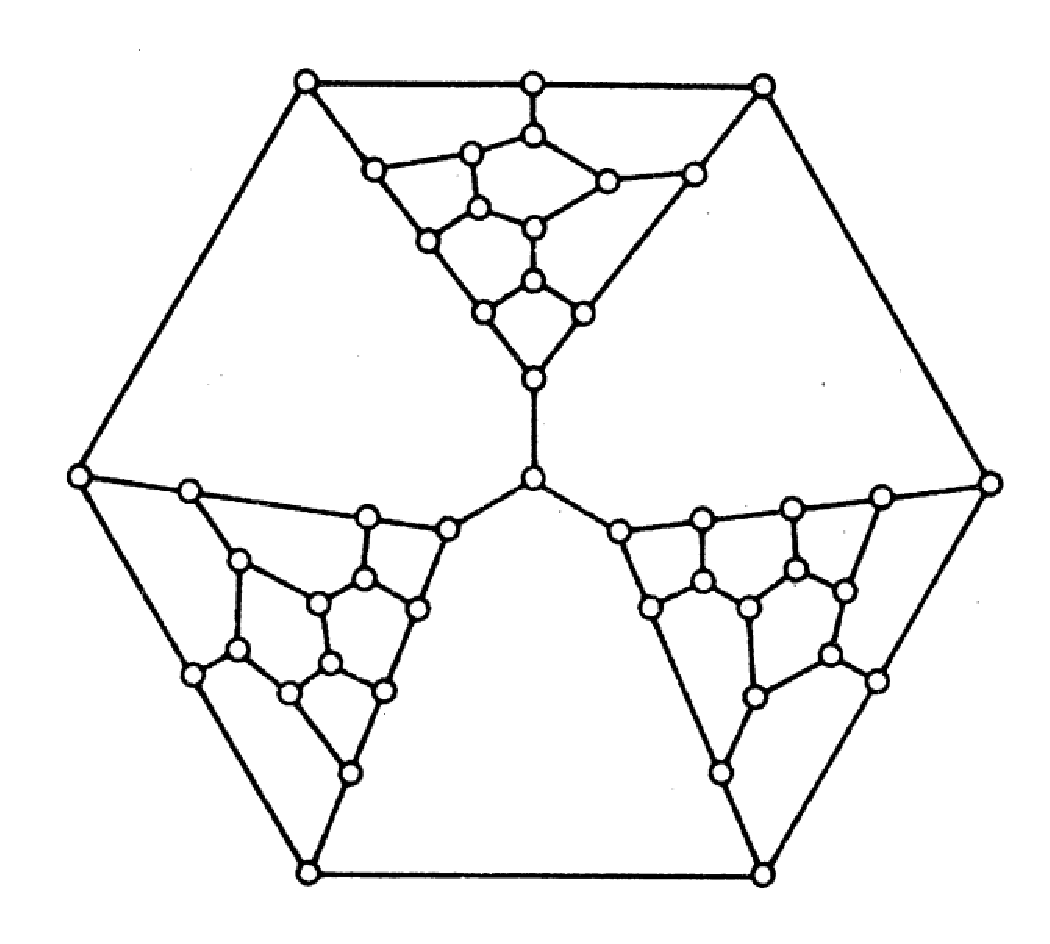
\includegraphics[width=7cm, height=6cm]{e4}
\end{frame}


\section{库拉托斯基定理}
\begin{frame}
  \frametitle{9.3 库拉托斯基定理、对偶图}
  \begin{Def}
    设$x=uv$为图$G=(V,E)$的一条边,又$w$不是$G$的顶点,则当用边$uw$和$wv$代替边$x$时,就称$x$被细分。如果$G$的某些条边被细分,产生的图称为$G$的细分图。
  \end{Def}
  \begin{Def}
    两个图称为同胚的,如果它们都可以从同一个图通过一系列的边细分得到。
  \end{Def}
  \begin{Thm}
    一个图为可平面的充分必要条件是它没有同胚于$K_5$或$K_{3,3}$的子图。
  \end{Thm}
\end{frame}
\begin{frame}
  \frametitle{9.3 库拉托斯基定理、对偶图}
  \begin{Def}
    一个图$G$的一个初等收缩由等同两个临接的顶点$u$和$v$得到,即从$G$中去掉$u$和$v$,然后再加上一个新顶点$w$,使得$w$临接于所有临接于$u$或$v$的顶点。一个图$G$可以收缩到图$H$,如果$H$可以从$G$经过一系列的初等收缩得到。
  \end{Def}
  \begin{Thm}
    一个图为可平面的当且仅当它没有一个可以收缩到$K_5$或$K_{3,3}$的子图。
  \end{Thm}
\end{frame}
\begin{frame}
  \frametitle{9.3 库拉托斯基定理、对偶图}
  \begin{Def}
    设$G=(V,E)$为一个平面图,由$G$按照如下方法构造一个图$G^*$,$G^*$称为$G$的对偶图:对$G$的每个面$f$对应地有$G^*$的一个顶点$f^*$;对$G$的每条边$e$对应地有$G^*$的一条边$e^*$:$G^*$的两个顶点$f^*$与$g^*$由边$e^*$联结,当且仅当$G$中与顶点$f^*$与$g^*$对应的面$f$与$g$有公共边$e$,如果某条边$x$仅在一个面中出现而不是两个面的公共边,则在$G^*$中这个面对应的顶点有一个环。
  \end{Def}
\end{frame}
\section{图的顶点着色}
% \begin{frame}
%   \frametitle{9.4 图的顶点着色}
%   \pause\centering
% \includegraphics[width=5cm,height=3cm]{Worldmap}
  % \begin{itemize}
  % \item A fights with B and E;
  % \item B fights with A and C;
  % \item C fights with B, E and F;
  % \item D fights with E;
  % \item E fights with A, C and D;
  %   \item F fights with C.
  % \end{itemize}
% \end{frame}
\begin{frame}
  \frametitle{9.4 图的顶点着色}
  \begin{Def}
    图的一种\alert{(顶点)着色}是指对图的每个顶点指定一种颜色,使得没有两个临接的顶点着同一种颜色。\pause图$G$的一个\alert{$n-$着色}是用$n$种颜色对$G$的着色。
  \end{Def}\pause
  \begin{Def}\justifying\let\raggedright\justifying
    图$G$的\alert{色数}是使$G$为$n-$着色的数$n$的最小值,图$G$的色数记为$\chi(G)$。\pause若$\chi (G) \leq n$,则称$G$为\alert{$n-$可着色}的。\pause若$\chi (G) = n$,则称$G$为\alert{$n$色}的。
  \end{Def}
\end{frame}
\begin{frame}
    \centering
  \begin{minipage}{0.24\linewidth}
    \centering
    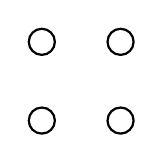
\begin{tikzpicture}[auto,
    specification/.style ={circle, draw, thick}]
   \node[specification] (A) at (0,0)  {};
   \node[specification] (B)  at (0,1)  {};
   \node[specification] (C)  at (1,1)  {};
   \node[specification] (D) at (1,0)  {};
 \end{tikzpicture}\\
 A
\end{minipage}\hfill 
  \begin{minipage}{0.24\linewidth}
    \centering
    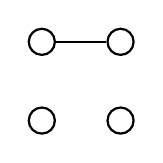
\begin{tikzpicture}[auto,
    specification/.style ={circle, draw, thick}]
   \node[specification] (A) at (0,0)  {};
   \node[specification] (B) at (0,1)  {};
   \node[specification] (C) at (1,1)  {};
   \node[specification] (D) at (1,0)  {};
   \draw[thick] (B) to  (C);
 \end{tikzpicture}\\
 B
\end{minipage}\hfill 
  \begin{minipage}{0.24\linewidth}
    \centering
    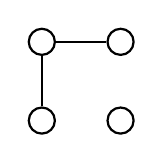
\begin{tikzpicture}[auto,
    specification/.style ={circle, draw, thick}]
   \node[specification] (A) at (0,0)  {};
   \node[specification] (B) at (0,1)  {};
   \node[specification] (C) at (1,1)  {};
   \node[specification] (D) at (1,0)  {};
   \draw[thick] (A) to  (B);
   \draw[thick] (B) to  (C);
 \end{tikzpicture}\\
 C
\end{minipage}\hfill 
  \begin{minipage}{0.24\linewidth}
    \centering
    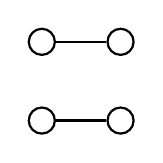
\begin{tikzpicture}[auto,
    specification/.style ={circle, draw, thick}]
   \node[specification] (A)  at (0,0)  {};
   \node[specification] (B)  at (0,1)  {};
   \node[specification] (C)  at (1,1)  {};
   \node[specification] (D) at (1,0)  {};
   \draw[thick] (B) to  (C);
   \draw[thick] (D) to  (A);
 \end{tikzpicture}\\
 D
\end{minipage}\hfill

\vspace*{0.5cm}
  \begin{minipage}{0.24\linewidth}
    \centering
    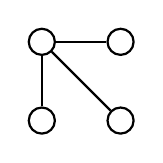
\begin{tikzpicture}[auto,
    specification/.style ={circle, draw, thick}]
   \node[specification] (A) at (0,0)  {};
   \node[specification] (B)  at (0,1)  {};
   \node[specification] (C)  at (1,1)  {};
   \node[specification] (D) at (1,0)  {};
   \draw[thick] (A) to (B);
   \draw[thick] (B) to (C);
      \draw[thick] (B) to (D);
 \end{tikzpicture}\\
 E
\end{minipage}\hfill
  \begin{minipage}{0.24\linewidth}
    \centering
    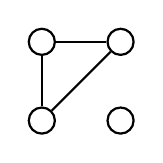
\begin{tikzpicture}[auto,
    specification/.style ={circle, draw, thick}]
   \node[specification] (A) at (0,0)  {};
   \node[specification] (B) at (0,1)  {};
   \node[specification] (C) at (1,1)  {};
   \node[specification] (D) at (1,0)  {};
   \draw[thick] (A) to  (B);
   \draw[thick] (B) to (C);
   \draw[thick] (C) to (A);
 \end{tikzpicture}\\
 F
\end{minipage}\hfill
  \begin{minipage}{0.24\linewidth}
    \centering
    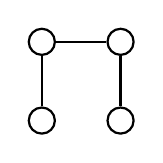
\begin{tikzpicture}[auto,
    specification/.style ={circle, draw, thick}]
   \node[specification] (A) at (0,0)  {};
   \node[specification] (B) at (0,1)  {};
   \node[specification] (C) at (1,1)  {};
   \node[specification] (D) at (1,0)  {};
   \draw[thick] (A) to  (B);
   \draw[thick] (B) to  (C);
      \draw[thick] (C) to (D);
 \end{tikzpicture}\\
 G
\end{minipage}\hfill 
  \begin{minipage}{0.24\linewidth}
    \centering
    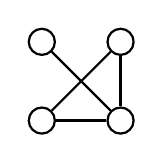
\begin{tikzpicture}[auto,
    specification/.style ={circle, draw, thick}]
   \node[specification] (A)  at (0,0)  {};
   \node[specification] (B)  at (0,1)  {};
   \node[specification] (C)  at (1,1)  {};
   \node[specification] (D) at (1,0)  {};
   \draw[thick] (A) to  (C);
   \draw[thick] (C) to  (D);
   \draw[thick] (D) to (A);
   \draw[thick] (B) to (D);
 \end{tikzpicture}\\
 H
\end{minipage}\hfill 

\vspace*{0.5cm}
\flushleft
  \begin{minipage}{0.24\linewidth}
    \centering
    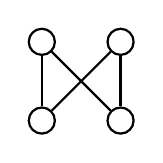
\begin{tikzpicture}[auto,
    specification/.style ={circle, draw, thick}]
   \node[specification] (A) at (0,0)  {};
   \node[specification] (B)  at (0,1)  {};
   \node[specification] (C)  at (1,1)  {};
   \node[specification] (D) at (1,0)  {};
   \draw[thick] (A) to (B);
   \draw[thick] (B) to (D);
   \draw[thick] (D) to (C);
      \draw[thick] (C) to (A);
 \end{tikzpicture}\\
 I
\end{minipage}
  \begin{minipage}{0.24\linewidth}
    \centering
    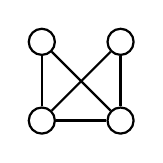
\begin{tikzpicture}[auto,
    specification/.style ={circle, draw, thick}]
   \node[specification] (A) at (0,0)  {};
   \node[specification] (B) at (0,1)  {};
   \node[specification] (C) at (1,1)  {};
   \node[specification] (D) at (1,0)  {};
   \draw[thick] (A) to  (B);
      \draw[thick] (C) to (D);
   \draw[thick] (D) to (A);
   \draw[thick] (A) to (C);
   \draw[thick] (B) to (D);
 \end{tikzpicture}\\
 J
\end{minipage} 
  \begin{minipage}{0.24\linewidth}
    \centering
    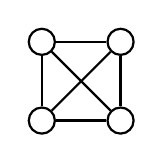
\begin{tikzpicture}[auto,
    specification/.style ={circle, draw, thick}]
   \node[specification] (A) at (0,0)  {};
   \node[specification] (B) at (0,1)  {};
   \node[specification] (C) at (1,1)  {};
   \node[specification] (D) at (1,0)  {};
   \draw[thick] (A) to  (B);
   \draw[thick] (B) to  (C);
      \draw[thick] (C) to (D);
   \draw[thick] (D) to (A);
   \draw[thick] (A) to (C);
   \draw[thick] (B) to (D);
 \end{tikzpicture}\\
 K
\end{minipage}  
\end{frame}

\begin{frame}
  \frametitle{9.4 图的顶点着色}
  \begin{Thm}
    一个图是可双色的当且仅当它没有奇数长的圈。
  \end{Thm}
\end{frame}

% \begin{frame}
%   \frametitle{9.4 图的顶点着色}
%   \begin{Thm}
%     一个图是可双色的当且仅当它没有奇数长的圈。
%   \end{Thm}
% \vspace{1cm}
%   \begin{minipage}{0.45\linewidth}
% \includegraphics[width=4cm,height=3cm]{pentagon}    
%   \end{minipage}
%   \begin{minipage}{0.45\linewidth}
   
%   \end{minipage}
% \end{frame}

% \begin{frame}
%   \frametitle{9.4 图的顶点着色}
%   \begin{Thm2}
%     一个图是可双色的当且仅当它没有奇数长的圈。
%   \end{Thm2}
% \vspace{1cm}
%   \begin{minipage}{0.45\linewidth}
% \includegraphics[width=4cm,height=3cm]{pentagon1}    
%   \end{minipage}
%   \begin{minipage}{0.45\linewidth}
   
%   \end{minipage}
% \end{frame}
% \begin{frame}
%   \frametitle{9.4 图的顶点着色}
%   \begin{Thm2}
%     一个图是可双色的当且仅当它没有奇数长的圈。
%   \end{Thm2}
% \vspace{1cm}
%   \begin{minipage}{0.45\linewidth}
% \includegraphics[width=4cm,height=3cm]{pentagon2}    
%   \end{minipage}
%   \begin{minipage}{0.45\linewidth}
   
%   \end{minipage}
% \end{frame}

% \begin{frame}
%   \frametitle{9.4 图的顶点着色}
%   \begin{Thm2}
%     一个图是可双色的当且仅当它没有奇数长的圈。
%   \end{Thm2}
% \vspace{1cm}
%   \begin{minipage}{0.45\linewidth}
% \includegraphics[width=4cm,height=3cm]{pentagon3}    
%   \end{minipage}
%   \begin{minipage}{0.45\linewidth}
   
%   \end{minipage}
% \end{frame}
% \begin{frame}
%   \frametitle{9.4 图的顶点着色}
%   \begin{Thm2}
%     一个图是可双色的当且仅当它没有奇数长的圈。
%   \end{Thm2}
% \vspace{1cm}
%   \begin{minipage}{0.45\linewidth}
% \includegraphics[width=4cm,height=3cm]{pentagon4}    
%   \end{minipage}
%   \begin{minipage}{0.45\linewidth}
   
%   \end{minipage}
% \end{frame}
% \begin{frame}
%   \frametitle{9.4 图的顶点着色}
%   \begin{Thm2}
%     一个图是可双色的当且仅当它没有奇数长的圈。
%   \end{Thm2}
% \vspace{1cm}
%   \begin{minipage}{0.45\linewidth}
% \includegraphics[width=4cm,height=3cm]{pentagon5}    
%   \end{minipage}
%   \begin{minipage}{0.45\linewidth}
   
%   \end{minipage}
% \end{frame}

% \begin{frame}
%   \frametitle{9.4 图的顶点着色}
%   \begin{Thm2}
%     一个图是可双色的当且仅当它没有奇数长的圈。
%   \end{Thm2}
% \vspace{1cm}
%   \begin{minipage}{0.45\linewidth}
% \includegraphics[width=4cm,height=3cm]{pentagon5}    
%   \end{minipage}
%   \begin{minipage}{0.45\linewidth}
%     \includegraphics[width=4cm,height=3cm]{color2}
%   \end{minipage}
% \end{frame}
% \begin{frame}
%   \frametitle{9.4 图的顶点着色}
%   \begin{Thm2}
%     一个图是可双色的当且仅当它没有奇数长的圈。
%   \end{Thm2}
% \vspace{1cm}
%   \begin{minipage}{0.45\linewidth}
% \includegraphics[width=4cm,height=3cm]{pentagon5}    
%   \end{minipage}
%   \begin{minipage}{0.45\linewidth}
%     \includegraphics[width=4cm,height=3cm]{color21}
%   \end{minipage}
% \end{frame}

% \begin{frame}
%   \frametitle{9.4 图的顶点着色}
%   \begin{Thm2}
%     一个图是可双色的当且仅当它没有奇数长的圈。
%   \end{Thm2}
% \vspace{1cm}
%   \begin{minipage}{0.45\linewidth}
% \includegraphics[width=4cm,height=3cm]{pentagon5}    
%   \end{minipage}
%   \begin{minipage}{0.45\linewidth}
%     \includegraphics[width=4cm,height=3cm]{color22}
%   \end{minipage}
% \end{frame}
% \begin{frame}
%   \frametitle{9.4 图的顶点着色}
%   \begin{Thm2}
%     一个图是可双色的当且仅当它没有奇数长的圈。
%   \end{Thm2}
% \vspace{1cm}
%   \begin{minipage}{0.45\linewidth}
% \includegraphics[width=4cm,height=3cm]{pentagon5}    
%   \end{minipage}
%   \begin{minipage}{0.45\linewidth}
%     \includegraphics[width=4cm,height=3cm]{color23}
%   \end{minipage}
% \end{frame}
% \begin{frame}
%   \frametitle{9.4 图的顶点着色}
%   \begin{Thm2}
%     一个图是可双色的当且仅当它没有奇数长的圈。
%   \end{Thm2}
% \vspace{1cm}
%   \begin{minipage}{0.45\linewidth}
% \includegraphics[width=4cm,height=3cm]{pentagon5}    
%   \end{minipage}
%   \begin{minipage}{0.45\linewidth}
%     \includegraphics[width=4cm,height=3cm]{color24}
%   \end{minipage}
% \end{frame}
% \begin{frame}
%   \frametitle{9.4 图的顶点着色}
%   \begin{Thm2}
%     一个图是可双色的当且仅当它没有奇数长的圈。
%   \end{Thm2}
% \vspace{1cm}
%   \begin{minipage}{0.45\linewidth}
% \includegraphics[width=4cm,height=3cm]{pentagon5}    
%   \end{minipage}
%   \begin{minipage}{0.45\linewidth}
%     \includegraphics[width=4cm,height=3cm]{color25}
%   \end{minipage}
% \end{frame}

% \begin{frame}
%   \frametitle{9.4 图的顶点着色}
%   \begin{Thm2}
%     一个图是可双色的当且仅当它没有奇数长的圈。
%   \end{Thm2}
% \vspace{1cm}
%   \begin{minipage}{0.45\linewidth}
% \includegraphics[width=4cm,height=3cm]{pentagon5}    
%   \end{minipage}
%   \begin{minipage}{0.45\linewidth}
%     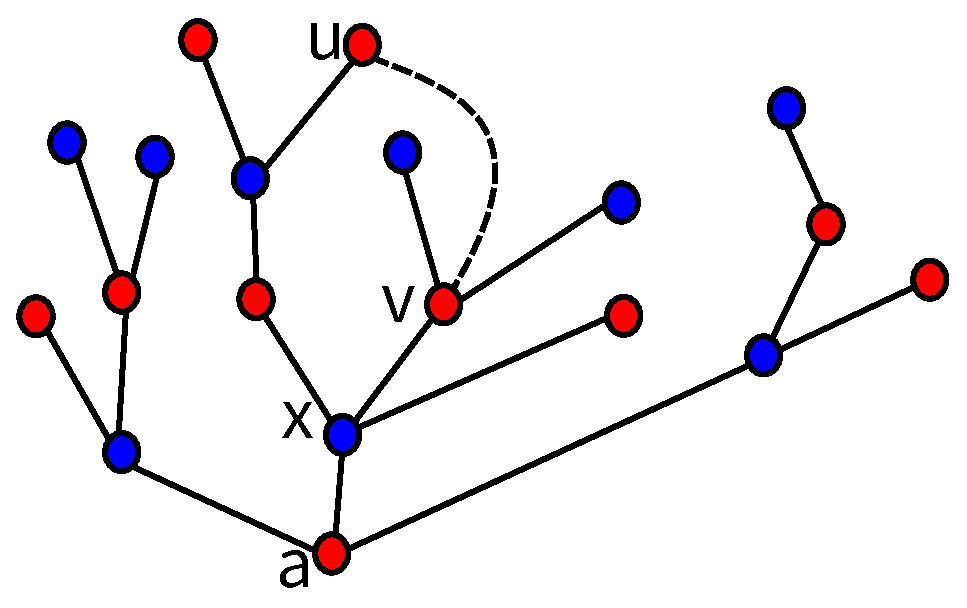
\includegraphics[width=4cm,height=3cm]{color26}
%   \end{minipage}
% \end{frame}

% \begin{frame}
%   \frametitle{9.4 图的顶点着色}
%   \begin{Thm2}
%     一个图是可双色的当且仅当它没有奇数长的圈。
%   \end{Thm2}
%   \begin{proof}[证明]
%     设图$G$为可双色的,则显然图$G$没有奇数长的圈。这是因为假设图$G$有奇数长的圈$C$,
%   则$C$是3色的,从而$\chi(G) \geq 3$,与$G$是可双色的矛盾。  
%   \end{proof}
% \end{frame}

% \begin{frame}
%   \frametitle{9.4 图的顶点着色}
%   \begin{Thm2}
%     一个图是可双色的当且仅当它没有奇数长的圈。
%   \end{Thm2}
%   \begin{proof}[证明(续上页)]
   

%   设图$G$没有奇数长的圈,以下给出一种用两种颜色对$G$的顶点进行着色的算法,从而证明图$G$是可双色的。不妨设图$G$是连通的,否则可以对图$G$的每个连通分量分别进行着色。任取$G$的一个顶点$a$,对其着红色,然后对与顶点$a$邻接的顶点着蓝色,接下来对所有与已经着色的顶点相邻接的顶点着红色,这样依次下去,每次都对所有与已经着色的顶点相邻接的顶点着与前一次的着色不同的另一种颜色。该算法结束时用至多两种颜色对$G$的顶点进行了着色。
  
%   \end{proof}
% \end{frame}
% \begin{frame}
%   \frametitle{9.4 图的顶点着色}
%   \begin{Thm2}
%     一个图是可双色的当且仅当它没有奇数长的圈。
%   \end{Thm2}
%   \begin{proof}[证明(续上页)]
%     以下证明每次对所有与已经着色的顶点相邻接的顶点着与前一次的着色不同的另一种颜色时,
% 不会产生相邻的两个顶点着以相同颜色的情况,从而保证前面的算法是正确的。用反证法。
% 假设对顶点$u$进行着色时,不妨设对其着红色,已经有一个与之相邻的顶点$v$着了红色。
% 从着色的过程知,从顶点$a$到顶点$u$之间有一条路$P_1$,其上的顶点依次着了红色和蓝色,
% 从顶点$a$到顶点$v$之间也有一条路$P_2$,其上的顶点依次着了红色和蓝色。
% 取$P_1$和$P_2$的最后一个公共的顶点$x$,则$P_1$上从顶点$u$到顶点$x$的路与$P_2$上从顶点$x$到顶点$v$的路和边$vu$一起构成一个圈,该圈上$u$和$v$着相同的颜色,其他各顶点依次着不同的颜色,因此其长度为奇数,与$G$中没有奇数长的圈矛盾。 
%   \end{proof}
% \end{frame}

\begin{frame}
  \frametitle{9.4 图的顶点着色}
  \begin{Thm}
    设$\Delta = \Delta (G)$为图$G$的顶点度的最大值,则$G$为$(\Delta+1)-$可着色的。
  \end{Thm}
 \pause \begin{proof}[证明]\justifying\let\raggedright\justifying
   \pause 用数学归纳法证明,\pause施归纳于顶点数$p$。

   \pause (1)当$p=1$时,结论显然成立。

   \pause (2)假设当$p=k(k\geq 1)$时结论成立,\pause往证当$p=k+1$时结论也成立。\pause设$v$为$G$中的任意一个顶点,\pause由归纳假设,\pause$G-v$是$\Delta(G-v)+1$可着色的。\pause又由于$\Delta(G-v) \leq \Delta$,\pause从而$G-v$为$\Delta+1$可着色的。\pause假设已经用至多$\Delta+1$种颜色对$G-v$进行了顶点着色,\pause使得任意相邻的顶点着不同的颜色,\pause那么此时在$G$中与$v$邻接的顶点用了至多$\Delta$种颜色,\pause用另外一种不同的颜色对顶点$v$进行着色,\pause从而用至多$\Delta+1$种颜色就可以对$G$的顶点进行着色使得相邻的顶点着不同的颜色,\pause即$G$为$\Delta + 1$可着色的。
  \end{proof}
\end{frame}
\begin{frame}
  \frametitle{9.4 图的顶点着色}
  \begin{Thm}
    如果$G$是一个连通图且不是完全图也不是奇数长的圈,则$G$为$\Delta(G)-$可着色的。
  \end{Thm}
\end{frame}
\begin{frame}
  \frametitle{9.4 图的顶点着色}
  \begin{Thm}
    每个平面图为$6-$可着色的。
  \end{Thm}
     \pause \begin{proof}[证明]\justifying\let\raggedright\justifying
   \pause 用数学归纳法证明,\pause施归纳于顶点数$p$。

   \pause (1)当$p=1$时,结论显然成立。

   \pause (2)假设当$p=k(k\geq 1)$时结论成立,\pause往证当$p=k+1$时结论也成立。\pause设平面图$G$有$k+1$个顶点,\pause则图$G$中一定有一个顶点$v$使得$\deg v \leq 5$。\pause于是,\pause$G-v$是一个有$k$个顶点的平面图,\pause由归纳假设,\pause$G-v$是$6-$可着色的。\pause假设用至多$6$种颜色对$G-v$进行了着色。\pause由于$\deg v \leq 5$,\pause在$G-v$中用至多$6$种颜色进行顶点着色时,\pause在$G$中与$v$邻接的顶点至多用了$5$种颜色。\pause此时,\pause用另外一种不同的颜色对顶点$v$进行着色,\pause这样用至多$6$种颜色就可以对$G$的顶点进行着色,\pause从而图$G$为$6-$可着色的。
  \end{proof}
\end{frame}
\begin{frame}
  \frametitle{9.4 图的顶点着色}
  \begin{Thm}
    每个平面图为$5-$可着色的。
  \end{Thm}
  \pause\begin{proof}[证明]\justifying\let\raggedright\justifying
  \pause用数学归纳法证明,\pause施归纳于图的顶点数$p$。

  \pause(1)当$p=1$时,\pause结论显然成立。

  \pause(2)假设当$p<k$时结论成立,\pause往证当$p=k$时结论也成立。\pause设平面图$G$有$k$个顶点,\pause则图$G$中一定有一个顶点$v$使得$\deg v \leq 5$。\pause于是,\pause$G-v$是一个有$k-1$个顶点的平面图,\pause由归纳假设,\pause$G-v$是$5-$可着色的。\pause假设用至多5种颜色对$G-v$进行了着色。\pause如果$\deg v \leq 4$,\pause则在$G-v$中用至多$5$种颜色进行顶点着色时,\pause在$G$中与$v$邻接的顶点至多用了$4$种颜色。\pause此时,\pause用另外一种不同的颜色对顶点$v$进行着色,\pause这样用至多5种颜色就可以对$G$的顶点进行着色,\pause从而图$G$为$5-$可着色的。

\renewcommand{\qedsymbol}{}    
\end{proof}

\end{frame}
\begin{frame}
  \frametitle{9.4 图的顶点着色}
  % \begin{Thm4.5}
  %   每个平面图为$5-$可着色的。
  % \end{Thm4.5}
{\small
  \begin{proof}[证明(续上页)]\justifying\let\raggedright\justifying
  \pause如果$\deg v = 5$,\pause与$v$邻接的$5$个顶点$v_1,v_2,v_3,v_4,v_5$在$G-v$中用$c_1,c_2,c_3,c_4,c_5$ 5种颜色进行了着色。\pause如果$c_1,c_2,c_3,c_4,c_5$中有两种颜色是相同的,\pause则$c_1$, $c_2$, $c_3$, $c_4$, $c_5$中至多有$4$种颜色,\pause用另外一种颜色对顶点$v$进行着色,\pause这样用至多5种颜色就可以对$G$的顶点进行着色。\pause以下考虑$c_1,c_2,c_3,c_4,c_5$中的各种颜色互不相同的情况。\pause在图$G$中,\pause与顶点$v$邻接的$5$个顶点$v_1,v_2,v_3,v_4,v_5$中一定有两个顶点是不邻接的,\pause否则图$G$中将有一个子图$K_5$,\pause这与图$G$为平面图相矛盾。\pause取其中不邻接的两个顶点$v_i$和$v_j$,\pause在$G-v$中,\pause将顶点$v_i$和顶点$v_j$视为同一个顶点$w$,\pause即去掉顶点$v_i$和$v_j$,\pause添加一个新的顶点$w$,\pause原来与顶点$v_i$和顶点$v_j$相关联的边变为与顶点$w$相关联的边,\pause得到的新的图记为$G'$,\pause则$G'$仍然为平面图。\pause由归纳假设,\pause$G'$为$5-$可着色的。 \pause设用至多$5$种颜色对$G'$进行了顶点着色。\pause在$G-v$中,\pause顶点$v_i$和顶点$v_j$都着与$w$相同的颜色,\pause其他的顶点均与$G'$中相对应的顶点着相同的颜色,\pause这样$G-v$用至多5种颜色就可以进行顶点着色。\pause在这里,\pause$G$中与顶点$v$邻接的五个顶点$v_1,v_2,v_3,v_4,v_5$中用了4种颜色,\pause用另外一种颜色对顶点$v$着色,\pause这样用至多5种颜色就可以对$G$的顶点进行着色,\pause从而图$G$为$5-$可着色的。
\end{proof}}

\end{frame}



% \begin{frame}
%   \frametitle{9.4 图的顶点着色}
%   \begin{Thm}
%     每个平面图为$5-$可着色的。
%   \end{Thm}
% \vspace{1cm}
% \includegraphics[width=4cm,height=3cm]{color52}
% \end{frame}
% \begin{frame}
%   \frametitle{9.4 图的顶点着色}
%   \begin{Thm3}
%     每个平面图为$5-$可着色的。
%   \end{Thm3}
% \vspace{1cm}
% \includegraphics[width=4cm,height=3cm]{color53}
% \end{frame}

% \begin{frame}
%   \frametitle{9.4 图的顶点着色}
%   \begin{Thm3}
%     每个平面图为$5-$可着色的。
%   \end{Thm3}
% \vspace{1cm}
% \includegraphics[width=4cm,height=3cm]{color51}
% \end{frame}

\begin{frame}
  \frametitle{9.4 图的顶点着色}
  \begin{Thm}
    每个平面图为$4-$可着色的。
  \end{Thm}
\end{frame}
\begin{frame}

  {\small
  \begin{Exercise}
    若$G$是一个$(p,q)$图,$q > \frac{1}{2}(p-1)(p-2)$,试证$G$是连通图。  
  \end{Exercise}}
  {\small
\pause\begin{proof}[证法一]\justifying\let\raggedright\justifying
      \pause用反证法。\pause假设$G$不连通,\pause则至少有两个支。\pause设其中一个支的顶点数为$p_1$,\pause边数为$q_1$,\pause所有其他支的顶点数为$p_2$,\pause边数为$q_2$。\pause则
    \begin{equation*}
      \begin{split}
       &\frac{1}{2}(p-1)(p-2)\\
        =&\frac{1}{2}(p_1 + p_2 -1)(p_1 + p_2 -2)\\
      =&\frac{1}{2}(p_1 + p_2 -1)((p_1 - 1) + (p_2 - 1))\\
      =&\frac{1}{2}(p_1(p_1 -1) +  p_1(p_2 - 1) + p_2(p_1 - 1) + p_2(p_2-1) - (p_1 - 1) - (p_2-1))\\
      =&\frac{1}{2}(p_1(p_1 -1) +   p_2(p_2-1) + 2(p_1 - 1)(p_2-1))\\
      =&\frac{p_1(p_1 -1)}{2} +   \frac{p_2(p_2-1)}{2} + (p_1 - 1)(p_2-1)\\
      \geq&\frac{p_1(p_1 -1)}{2} +   \frac{p_2(p_2-1)}{2}
       \geq  q \quad \text{矛盾。}
      \end{split}
    \end{equation*}
    
\end{proof}}
\end{frame}
\begin{frame}
  \begin{Exercise}
    若$G$是一个$(p,q)$图,$q > \frac{1}{2}(p-1)(p-2)$,试证$G$是连通图。  
  \end{Exercise}
\pause\begin{proof}[证法二]\justifying\let\raggedright\justifying
  \pause用反证法。\pause假设$G$不连通,\pause则至少有两个支。\pause设其中一个支为$G_1=(V_1,E_1)$,包含$p_1$个顶点,$q_1$条边,\pause其余的支构成的子图为$G_2=(V_2,E_2)$,包含$p_2$个顶点,$q_2$条边。
  \pause则$G_1$中的边数与$G_2$中的边数之和小于等于$K_{p_1}$和$K_{p_2}$中的边数之和。\pause将$K_{p_1}$和$K_{p_2}$视为一个图,\pause取$K_{p_1}$中的一个顶点$u$和$K_{p_2}$中的一个顶点$v$,\pause将$K_{p_1}$中与$u$相关联的边替换为与$v$相关联的边(边的另一个顶点保持不变)所得到的子图为$G'$,\pause则$K_{p_1}$和$K_{p_2}$中的边数之和等于$G'$中的边数。\pause显然$G'$中的边数小于等于$K_{p-1}$中的边数,\pause从而$G_1$中的边数与$G_2$中的边数之和小于等于$K_{p-1}$中的边数,即
  \[q\leq \frac{1}{2}(p-1)(p-2)\]
  矛盾。
\end{proof}
\end{frame}
\begin{frame}
  \begin{Exercise}
  证明:如果图$G$不是连通图,则$G^c$是连通图。
\end{Exercise}
\pause\begin{proof}[证明]\justifying\let\raggedright\justifying
  \pause设$u$和$v$为$G^c$中的任意两个不同的顶点。\pause如果$u$和$v$不在$G$的同一个连通分量中,\pause则$uv$不是$G$的一条边,\pause于是$uv$为$G^c$的一条边,\pause从而在$G^c$中$u$和$v$之间存在一条路;\pause如果$u$和$v$在$G$的同一个连通分量中,\pause取$G$的另外一个连通分量中的一个顶点$w$,\pause则$uw$和$wv$都不是$G$中的边,\pause从而为$G^c$中的边,\pause于是$uwv$构成了$G^c$中$u$和$v$之间的一条路。
\end{proof}
\end{frame}
\begin{frame}
    \begin{Exercise}
  证明:一个连通的$(p,q)$图中$q\geq p - 1$。  
  \end{Exercise}
  \begin{proof}[证明]
    设$G$为一个连通图,有$p$个顶点,$q$条边。如果$G$中有圈,去掉该圈上的一条边,得到的图仍然为连通的。如果所得到的图中还有圈,再去掉该圈上的一条边,得到的图还是连通的。如此进行下去,最后可以得到一个连通无圈的图。假设该连通无圈的图中有$q'$条边,如果能够证明$q'=p-1$,则结论得证。

    因此,只需证明一个连通无圈的$(p,q)$图中$q=p-1$即可。设$T$为一个连通无圈的$(p,q)$图,以下用数学归纳法证明$q=p-1$。
  \end{proof}
\end{frame}
\begin{frame}
  \begin{proof}[证明]
  
    用数学归纳法证明,施归纳于顶点数$p$。
    
    (1)当$p=1$时,$q=0$,结论显然成立。

    (2)假设当$p=k$时结论成立,往证当$p=k+1$时结论也成立。设$T$有$k+1$个顶点。$T$中一定存在一个度为1的顶点,这是因为,设$P$为$T$中的一条最长
    路,$v$为$P$的一个端点,则$v$除了$P$上与其关联的边之外,由$T$中无圈知$v$不能再有其他的与$P$上的顶点相关联的边,同时由$P$为一条最长路知$v$不能再有与$P$外
    的顶点相关联的边,因此$v$的度必为1。去掉$T$中一个度为1的顶点及其与之关联的边,得到的图$T'$连通且无圈。$T'$有$k$个顶点,$q-1$条边,由归纳假设,$q-1 = k - 1$, 从而$q = (k +1) - 1$, 即当$p=k+1$时结论也成立。
  \end{proof}
\end{frame}

\begin{frame}
\begin{proof}[证明]
        用数学归纳法证明,施归纳于边数$q$。
    
    (1)当$q=0$时,$p=1$,结论显然成立。

    (2)假设当$q<k$时结论成立,往证当$q=k$时结论也成立。设$T$有$k$条边。去掉
    $T$中的任意一条边,得到两个支$T_1$和$T_2$,它们均连通无圈。设$T_1$有$p_1$个顶点,
    $k_1$条边,$T_2$有$p_2$个顶点,$k_2$条边,由归纳假设,
    \begin{equation*}
      \begin{split}
        k_1 &= p_1 - 1\\
        k_2 &= p_2 - 1
      \end{split}
    \end{equation*}
    以上两式相加,两边再同时加1,得
    \[k_1 + k_2  + 1 = p_1 + p_2 - 1\]
    从而
    \[k = p - 1 \]
    即当$q=k$时结论也成立。
\end{proof}
\end{frame}
\begin{frame}
  \begin{Exercise}
    若$G$是一个$(p,q)$图,$q > \frac{1}{2}(p-1)(p-2)$,试证$G$是连通图。  
  \end{Exercise}
\pause\begin{proof}[证法三]\justifying\let\raggedright\justifying
  \pause用反证法。\pause假设$G$不连通,\pause则$G^c$连通,\pause从而$G^c$中的边数$q'\geq p-1$,\pause于是$G$中的边数$q\leq \frac{1}{2}p(p-1)-(p-1)=\frac{1}{2}(p-1)(p-2)$,
  \pause矛盾。
\end{proof}
\end{frame}

\begin{frame}
  \begin{Exercise}
    恰有两个顶点不是割点的连通图是一条路。
  \end{Exercise}
  \pause\begin{proof}[证明]\justifying\let\raggedright\justifying\pause设连通图$G$有$p$个顶点,\pause恰有两个顶点不是割点,\pause往证$G$为一条路。\pause由$G$连通知,\pause $G$有一棵生成树$T$。\pause取树$T$的一条最长路$P:v_1v_2\cdots v_k$,\pause则$v_1$和$v_k$在$T$中的度必为$1$,\pause它们都不是$T$的割点,\pause从而也不是图$G$的割点。\pause由$G$中恰有两个顶点不是割点知,\pause$T$中除了$v_1$和$v_k$之外没有其他度为$1$的顶点,\pause由此可得出$T$中所有顶点的度小于等于$2$。\pause否则,\pause假设$T$中存在一个度大于等于$3$的顶点,\pause则$T$中所有顶点的度数之和$\geq 3 + 2 + 2(p-3) = 2p -1 > 2(p-1)$,\pause矛盾。\pause由$T$中所有顶点的度小于等于$2$知,\pause路$P$中包含了$T$中所有的顶点,\pause即路$P$中包含了$G$中所有的顶点。\pause事实上,\pause $G$就是路$P$。\pause否则,\pause在路$P$中,\pause设$v_i$和$v_j$($j>i+1$)之间在$G$中有一条边,\pause则$v_{i+1}$不是$G$的割点,\pause与$G$中只有两个顶点$v_1$和$v_k$不是割点矛盾。
  \end{proof}
\end{frame}
\begin{frame}
  \begin{Exercise}
    证明:若$G$的任两个奇数长的圈都有一个公共顶点,则$\chi(G)\leq 5$。
  \end{Exercise}
  \pause\begin{proof}[证明]\justifying\let\raggedright\justifying
  \pause用反证法,\pause假设$\chi(G)=n$, $n \geq 6$。\pause对图$G$的顶点用$n$种颜色进行着色,\pause使得任意两个相邻的顶点着不同的颜色。
  \pause设$V_1$,$V_2$,$V_3$为其中着3种不同颜色的顶点集合,\pause$V_4$,$V_5$,$V_6$为其中着另外3种不同颜色的顶点集合。\pause则由$V_1\cup V_2\cup V_3$导出的子图$G_1$不是2-可着色的,\pause从而$G_1$中存在一个奇数长的圈$C_1$;\pause同理,由$V_3\cup V_4\cup V_6$导出的子图$G_2$中存在一个奇数长的圈$C_2$。\pause$C_1$和$C_2$没有公共顶点,\pause矛盾。
\end{proof}
\end{frame}
\begin{frame}
  \begin{Def1}
    针对$\cup$,$\cap$,$^c$运算,递归的定义集合表达式如下:

    1)单独的集合符号为集合表达式

    2)如果$A$为集合表达式,则$A^c$为集合表达式;如果$A$与$B$为集合表达式,则$A\cup B$,$A\cap B$都为集合表达式。
  \end{Def1}
\end{frame}
\begin{frame}
  \begin{Thm4}
    对于任意的集合表达式$E$,将式中的每个单独的集合符号$X$替换成$X^c$,将式中出现的$\cup$和$\cap$分别替换成$\cap$和$\cup$,得到的集合表达式记为$E'$,则$E^c=E'$。
  \end{Thm4}

  \pause如果$E\subseteq F$,则$E^c\supseteq F^c$,即$E'\supseteq F'$;

  \pause如果$E\supseteq F$,则$E^c\subseteq F^c$,即$E'\subseteq F'$;

  \pause如果$E=F$,则$E^c=F^c$,即$E'=F'$。
\end{frame}

\begin{frame}
  \begin{Thm4}
    对于任意的集合表达式$E$,将式中的每个单独的集合符号$X$替换成$X^c$,将式中出现的$\cup$和$\cap$分别替换成$\cap$和$\cup$,得到的集合表达式记为$E'$,则$E^c=E'$。
  \end{Thm4}
  \pause\begin{proof}[证明]\justifying\let\raggedright\justifying
    \pause用数学归纳法证明,\pause施归纳于集合表达式$E$中出现符号$\cup$,$\cap$和$^c$的次数$n$。

    \pause(1)当$n=0$时,\pause$E$中只出现了一个单独的集合,\pause设为$A$,\pause则$E^c=A^c$,\pause即$E^c=A'$。

    \pause(2)假设当$n<k$时结论成立,\pause往证当$n=k$时结论也成立。\pause设集合表达式$E$中出现了$k$个符号。\pause如果$E=A^c$,\pause则$A$中出现了$k-1$个符号,\pause由归纳假设,\pause $A^c=A'$。\pause此时,\pause$(A^c)^c=(A')^c$,\pause即$E^c=E'$。\pause如果$E=A\cup B$,\pause则$A$中和$B$中出现的符号数小于$k$,\pause由归纳假设,\pause$A^c=A'$,\pause$B^c=B'$。\pause此时,\pause$(A\cup B)^c=A^c\cap B^c=A'\cap B'$,\pause即$E^c=E'$。\pause如果$E=A\cap B$,\pause则$A$和$B$中出现的符号数小于$k$,\pause由归纳假设,\pause$A^c=A'$,\pause$B^c=B'$。\pause此时,\pause$(A\cap B)^c=A^c\cup B^c=A'\cup B'$,\pause即$E^c=E'$。
  \end{proof}
\end{frame}

\end{CJK}
\end{document}

%%% Local Variables:
%%% mode: latex
%%% TeX-master: t
%%% End:
